\chapter{Introduction}

\section{Research Context}

\begin{figure}[t]
    \centering
    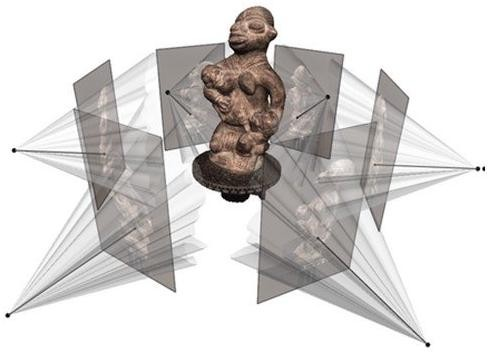
\includegraphics[width=0.72\linewidth]{res/01_introduction/image1.png}
    \caption{The multi-view principle underlying image-based 3D reconstruction. A set of
    calibrated cameras observes the same object from many directions; each camera records a
    single two-dimensional projection (its image plane and view frustum are shown), and it is
    the \emph{parallax} between these overlapping views that makes recovering the underlying
    three-dimensional structure possible. This same principle is the foundation on which both
    static 3D Gaussian Splatting and the dynamic, fixed-camera extension developed in this
    thesis are built.}
    \label{fig:multiview}
\end{figure}

The precise three-dimensional reconstruction of indoor environments is a massive challenge in computer vision, with a long history that spans classical photogrammetry, geometric multi-view stereo, implicit neural fields, and the most recent generation of explicit radiance-field representations. The central question has remained unchanged over that time. Given a finite number of two-dimensional observations of a scene, can we recover a three-dimensional description accurate enough, so re-rendering the scene from viewpoints that were never actually captured is possible (Figure~\ref{fig:multiview})? This thesis focuses on \textbf{reconstructing indoor environments that contain motion}, using only multi-view RGB video, and producing a representation that can be rendered in real time. The motivating application is broader than computer graphics. There is a growing interest among experimental psychologists and behavioural researchers in digital twins of indoor spaces as testing environments for cognitive experiments. A digital twin of a room that preserves not only its static geometry and appearance but also the movement of its subjects opens the door to reproducible behavioural paradigms where a participant's movements and decision-making can be studied against a 4D environment. For such use cases the accuracy of the reconstruction is not a matter of aesthetics, it is a prerequisite for the validity of the experiment. The technical backbone of the proposed pipeline is \emph{3D Gaussian Splatting (3DGS)} \cite{kerbl2023}, an explicit, point-based, differentiable radiance-field representation that has established itself as the dominant alternative to Neural Radiance Fields since 2023. Static 3DGS is a solved problem in the sense that the reference implementation converges reliably and renders at over 100\,FPS on consumer GPUs. The situation in the temporal domain is far less settled, a handful of extensions exist, but they disagree on the most basic design choices, and none is obviously well-suited to the characteristic properties of indoor video captures, namely mostly rigid background geometry, comparatively sparse moving content (one or two human actors), static cameras, and capture durations in the tens of seconds rather than a few frames.

The specific regime targeted here is narrower than dynamic-scene reconstruction in general, and that narrowness is deliberate. A behavioural laboratory is a fixed room, instrumented once with a small set of cameras attached to the walls or ceiling; the cameras do not move during a session, the lighting is controlled, and the only thing that changes from frame to frame is the participant moving through the space. Most of every image is therefore identical across the entire capture, and the moving content is confined to one or two people occupying a small fraction of the volume. A method built for arbitrary, in-the-wild video has to spend its capacity coping with moving cameras, changing illumination, and dense motion that none of these captures exhibit, and it pays for that generality in training time, storage, and complexity. The central wager of this thesis is that, by taking the constraints of this regime seriously instead of treating them as a special case of the general problem, a markedly simpler method can match or exceed the general-purpose machinery while remaining cheap to train, compact to store, and trivial to render.

This thesis proposes and evaluates an extension of 3DGS to dynamic indoor scenes based on the explicit recognition that indoor videos naturally decompose into a \emph{static} component and a \emph{dynamic} component. The key insight is that this decomposition does not require any \emph{learned} segmentation network. The moving foreground is isolated by a model-free \emph{background subtraction}, a plain pixelwise comparison of each frame against a photograph of the empty room, while the static and dynamic partition of the Gaussian primitives themselves emerges from the optimisation, provided that the Gaussian topology is fixed after the first frame and that only the geometric parameters (position, scale, rotation, opacity) are allowed to evolve in time, with appearance held constant. The rest of the thesis develops this idea into a complete pipeline, implemented as a first-class method inside the \emph{nerfstudio} framework, evaluates it on a controlled synthetic benchmark with pixel-exact ground truth, and contrasts it with the most closely related prior work.

\section{Problem Statement: The Temporal Challenge in Neural Rendering}

While static 3DGS produces good reconstructions of stationary indoor geometry, extending the method to a temporal sequence raises four related algorithmic difficulties, on top of one methodological requirement on the input data discussed at the end of this section.

\begin{itemize}
    \item \textbf{Computational cost of per-frame reconstruction.} The most straightforward temporal extension of 3DGS is to treat each video frame as an independent scene and run the full static optimisation pipeline for every frame. With $T$ frames and the default $30\,000$ iterations per frame, a one-minute capture at $30$\,fps would require $5.4 \times 10^{7}$ optimiser steps. This would be highly inefficient on a single GPU, since the vast majority of the scene (the static background) is re-learned from scratch at every time step.

    \item \textbf{Loss of inter-frame correspondence.} A second naive approach is to re-initialise each frame from the previously trained one. This halves the training time, but under free optimisation (with densification, pruning, and colour updates enabled) there is no guarantee that the same physical feature continues to be represented by the same Gaussian across time. Any application that requires a trajectory (tracking a hand, re-timing a motion, extracting a dynamic object) immediately fails.

    \item \textbf{Degeneracies of fully free temporal optimisation.} When a per-frame 3DGS optimiser is given complete freedom, it can explain motion in two different ways: by \emph{moving} splats (geometrically correct) or by \emph{repainting} splats (geometrically wrong but photometrically cheap). In practice the loss landscape frequently funnels the optimiser toward the latter, producing reconstructions where moving subjects appear as smeared paintings on the static background rather than as objects with coherent 3D shape. This degeneracy, referred to in the thesis as \emph{colour-hallucinated motion}, is a direct consequence of allowing the spherical-harmonic coefficients to change in time.

    \item \textbf{Storage and memory growth.} Finally, a per-frame representation must be serialised somewhere. Unconstrained approaches produce one independent Gaussian field per frame, which grows memory linearly with $T$ \emph{and} with the splat count, since the splat count can itself grow from frame to frame under densification. At video lengths relevant to behavioural experiments (tens of seconds, thousands of frames) this becomes untenable.

\end{itemize}

A fifth difficulty is methodological rather than algorithmic, but it shapes the whole data pipeline: the input camera poses must be \emph{exact}. In a static capture a small pose error merely blurs the result, but in a dynamic capture it is far more insidious, because a pose error and a genuine scene motion produce the same kind of image change, a displacement of features, and are therefore indistinguishable to a tracker. Any error in the estimated poses would be silently re-interpreted as movement and would corrupt the very quantity the method is trying to measure. This is precisely the regime in which the classical Structure-from-Motion pipeline (such as COLMAP) becomes a liability rather than an asset, and it motivates the decision, developed in Chapter~3, to obtain poses by direct export from the synthetic scene rather than by estimation.

Existing four-dimensional extensions of 3DGS (see Section~2.4) address the temporal issues with varying degrees of success but converge on the same family of solutions: encode each Gaussian's time-dependence with an auxiliary neural network \cite{yang2024deformable}, a high-dimensional basis \cite{wu20244dgs}, or a per-Gaussian polynomial \cite{li2024spacetime}. All of these inject \emph{additional} machinery, with its own training dynamics and its own failure modes. The thesis asks whether a simpler, almost machinery-free solution is sufficient for the specific regime of indoor captures with static cameras.

\section{Research Objectives and Questions}

The primary objective of this thesis is to design, implement, and evaluate a dynamic extension of 3D Gaussian Splatting suitable for indoor multi-view video, and to understand the specific role played by each design choice. The work is organized around four research questions:

\begin{itemize}
    \item \textbf{Q1: System Structure.} Can a dynamic indoor scene be accurately reconstructed by establishing a fixed baseline on the first frame and directly tracking movement thereafter, without relying on complex neural networks?

    \item \textbf{Q2: Physical Accuracy.} Does locking the color and lighting variables (spherical harmonics) during the tracking phase force the system to capture true physical movement, rather than "faking" motion by merely shifting colors?

    \item \textbf{Q3: Computational Efficiency.} How much does predicting movement based on the previous frame's velocity (a linear, constant-velocity warm start) reduce the processing time and computational effort needed for each new frame?

    \item \textbf{Q4: Temporal Stability.} Under a fixed primitive budget, splats that drift off the subject are never replaced and the reconstruction slowly erodes over a long sequence. Can purely geometric, model-free constraints (restricting the photometric loss to the object silhouette and re-anchoring stray splats onto the subject's per-frame visual hull) prevent this drift without any learned priors?

\end{itemize}

Each of these questions is answered by a controlled comparison rather than by a single end-to-end score. The design choice under test is switched on and off while everything else is held fixed, and the quantity it is supposed to affect is measured directly: steps to convergence for the efficiency of velocity prediction, object-region fidelity and background leakage for the effect of frozen appearance and of the geometric constraints, and the stability of the per-primitive correspondence for the soundness of the tracking structure. Because the synthetic benchmark supplies exact ground truth, these comparisons attribute an observed change to the individual mechanism under study and not to the confounds that a real capture would introduce.

A secondary, methodological objective is to build the evaluation infrastructure that lets these questions be answered with confidence rather than asserted. This means chiefly the controllable synthetic dataset with pixel-exact ground-truth poses, but also the surrounding tooling that turns the method into a complete and reproducible pipeline: the model-free segmentation and visual-hull seeding that initialise the dynamic reconstruction; the dynamic method itself, implemented as a first-class \texttt{ns-train} method inside \emph{nerfstudio} so it inherits that framework's data management, checkpointing, and live web viewer; a \emph{viser}-based merge renderer that composites the static background with the per-frame dynamic foreground and plays the result back in real time; a unified per-frame PLY output format loadable by standard 3DGS tools; and a temporal compressor that exploits the fixed topology to shrink the per-frame sequence by roughly an order of magnitude.

\section{Summary of Contributions}
\label{sec:contributions}

Pulling the objectives together, the thesis makes the following concrete contributions, which the chapters that follow develop and evaluate in turn.

\begin{itemize}
    \item \textbf{A reproducible synthetic benchmark for dynamic indoor capture.} A furnished room is modelled and rendered in Blender, with the camera intrinsics and extrinsics exported directly from the scene. Because the poses are known exactly rather than estimated, the residual error of a reconstruction can be attributed to the reconstruction algorithm itself and not to calibration noise, which is what makes a fair study of the tracking quality possible at all.

    \item \textbf{A model-free foreground segmentation.} The moving subject is isolated onto a black background by background subtraction, using only a photograph of the empty room and a per-pixel comparison. No learned segmentation network appears anywhere in the pipeline, which removes an external, separately-trained dependency that the rest of the system would otherwise inherit.

    \item \textbf{The core algorithmic contribution, \texttt{temporal-splatfacto}.} A dynamic extension of 3D Gaussian Splatting that fits a single dense cloud on the first frame and then tracks it through the rest of the sequence under a fixed primitive count and frozen appearance. The tracking is stabilised by three model-free mechanisms: silhouette supervision that prevents primitives from drifting into the background, a linear velocity prediction that warm-starts each frame, and a per-frame re-anchoring of stray primitives to the subject's visual hull.

    \item \textbf{A real-time renderer and a temporal compressor.} A merge renderer composites the static background reconstruction with the per-frame dynamic foreground for interactive playback, while a temporal compressor exploits the constant topology to reduce the size of the per-frame sequence by roughly an order of magnitude with little loss of fidelity.

    \item \textbf{An ablation-style empirical study.} Rather than reporting a single aggregate number, the evaluation isolates the contribution of each design choice, quantifying separately the effect of velocity prediction on convergence speed, of frozen appearance on physical correctness, and of the geometric constraints on temporal stability.
\end{itemize}

\section{Scope and Limitations}

To keep the study focused and the conclusions meaningful, its scope is bounded by several deliberate design choices and restrictions. Primarily, the research exclusively uses temporally synchronized multi-view RGB video from fixed cameras. By intentionally omitting depth sensors such as LiDAR or RGB-D, the study stress-tests a purely vision-based pipeline and ensures that the contributions remain compatible with low-cost, camera-only capture rigs. Because the per-frame tracking assumes that the multi-view geometry does not change over the capture, the cameras must remain entirely static; the method exploits, rather than tolerates, this fixed rig, and the model-free segmentation additionally assumes a per-camera photograph of the empty room is available as a background plate.

Furthermore, the system is designed strictly for indoor scenes under controlled lighting, explicitly excluding outdoor illumination, strong shadows, and weather variations. Within these controlled spaces, the dynamic content is expected to consist of one or a few moving actors or displaced rigid objects. Complex volumetric or semi-transparent phenomena, such as fluid simulations, smoke, fire, or water are not modeled, as they violate the method's assumption that a surface maintains a stable reflectance over time. This is the same assumption that licenses freezing the appearance of every primitive after the first frame, so the two restrictions are really one.

Finally, the study's evaluation and processing regimes are tightly constrained. Evaluation is conducted within a fully synthetic environment rendered in Blender, which provides analytical ground truth for both camera poses and geometry. This approach isolates the method's performance from the noise present in real-world photogrammetric calibration; validation on physically captured footage is left to future work. The entire pipeline runs offline. Although the final output achieves real-time rendering frame rates, the training process and the per-frame tracking stage (which relies on a short optimization loop rather than a closed-form update) are computationally heavy and are not designed for real-time execution.

\section{Thesis Structure}

\noindent
The thesis is organised into four chapters.

\paragraph{Chapter 2: Literature Review and Theoretical Foundations.} This chapter goes over the evolution of 3D reconstruction from the geometric era (8-point algorithm, factorisation, COLMAP) through the implicit-neural era (NeRF, Instant-NGP) to the current radiance fields era (3D Gaussian Splatting). A dedicated section covers the emerging literature on dynamic and four-dimensional neural rendering (D-NeRF, Deformable 3DGS, 4D-GS, SpaceTime Gaussians, Dynamic 3D Gaussians), which provides the direct comparison baseline for the proposed method. The chapter closes with the formal mathematical background for the two pillars the work draws on. The first is COLMAP's incremental Structure-from-Motion pipeline, the classical route to camera poses, which the proposed method ultimately bypasses; the second is the differentiable rasterisation of 3DGS, which it extends.

\paragraph{Chapter 3: Research.} This chapter presents the full end-to-end pipeline. It begins with the construction of the synthetic evaluation environment in Blender (the parametric background-capture trajectory, the fixed-camera rig, and the exact intrinsics and extrinsics exported directly from the scene rather than estimated by Structure-from-Motion), together with the model-free background subtraction that isolates the moving subject. It then develops the two reconstruction branches: a reference static 3DGS reconstruction of the room, and the proposed dynamic extension, \texttt{temporal-splatfacto}, which combines visual-hull initialisation, a dense first-frame fit, and constrained per-frame tracking (constant topology, frozen appearance, silhouette supervision, linear velocity prediction, and per-frame hull snapping). It describes the merge renderer that composites the two components for real-time playback and the temporal compressor that exploits the fixed topology, and concludes with benchmarks quantifying the effect of each design choice.

\paragraph{Chapter 4: Conclusions.} Summarises the findings, discusses the limitations encountered during implementation and evaluation, and outlines ideas for future work.
